\clearpage
\section{Praxis}
\label{sec:practice}

Um die Schlussfolgerungen aus dem Forschungsteil weiter zu untersuchen, wurde sich dazu entschieden, die Vor- und Nachteile der Lerntypen in einem praktischen Selbstexperiment zu untersuchen.
Hierzu werden die Hänge in den einzelnen Lerndimensionen des Autors untersucht. Anschließend wird ein einfacher Algorithmus in einer funktionalen Programmiersprache umgesetzt. Es wurde sich in diesem Fall für Haskell entschieden, da es die meistverwendete funktionale Programmiersprache in Einsteiger Kursen im Bereich Informatik ist (siehe \nameref{sec:curriculares}).
Als Problem wurde "Türme von Hanoi" gewählt, ein klassisches Problem mit Backtracking.
Für das Problem wurde sich entschieden, da alle Aspekte von Computational Thinking (CT) gut vertreten sind, und wichtige Aspekte des funktionalen Programmierens wie Backtracking und Rekursion für die Lösung benötigt werden.
Das Problem ist zudem Teil des Kurses CIS 194 \cite{cis194} der University of Pennsylvania, der in der offiziellen Haskell Dokumentation empfohlen wird \cite{haskelldoc}. Der Kurs wurde im Rahmen der Bachelorarbeit verwendet, um die Grundkonzepte von Haskell zu erlernen, und durch praktische Übungen anzuwenden.

Weitere Erläuterungen zu der Art des Problemes folgen in Abschnitt \nameref{sec:problemdesc}.

\subsection{Lerntypenanalyse}
Um das Selbstexperiment in Verbindung mit den Vor- und Nachteilen der Lerntypen in den verschiedenen Feldern setzen zu können, musste zunächst eine eigene Lerntypen Analyse durchgeführt werden.
Hierzu wurde der "Index of Learning Styles Questionnaire" Fragebogen verwendet \cite{ils_questionnaire}, ein Online Tool welches insgesamt 44 Fragen stellt, und dann auf Basis der Antworten die Lerntypen eines Individuums einschätzen kann. Die Lerntypen, die als Gegensatzpaare definiert sind, befinden sich auf einer 2 Dimensionalen Skala, die einschätzen soll, wie ausgeprägt der Hang zu einem Aspekt ist. Ein Wert von 1 bis 3 entspricht einer ausgewogenen Balance beider Aspekte der Dimension. Ein Wert von 5 bis 7 entspricht einem mäßigem Hand zu einem Aspekt. Ein Wert von 9 bis 11 entspricht einer starken Präferenz eines Lernstiles in der Dimension.
Die Verlässlichkeit dieses Fragebogens wurde mehrmals, sowohl von den ursprünglichen Autoren des Lernmodelles \cite{felder2005}, als auch von anderen Quellen \cite{zywno}, geprüft und bestätigt.

\subsubsection{Ergebnisse der persönlichen Evaluierung}
Die Fragen des ILS Fragebogens wurden in einer zufälligen Reihenfolge beantwortet, um zu vermeiden, dass bereits vorab klar ist, welche Frage welcher Typendimension korrespondiert. Dies ist möglich, da der Test so aufgebaut ist, dass jeweils ein Frageblock von 4 Fragen jede Dimension behandelt. Die erste Frage beispielsweise geht in die Wertung der Aktiv/Reflektiven Dimension ein, die 5 Frage beschäftigt sich wieder mit der Dimension, und die 9 Frage ebenfalls.

Die Ergebnisse des Fragebogens lauten wie folgt.

\begin{figure}[H]
    \centering
    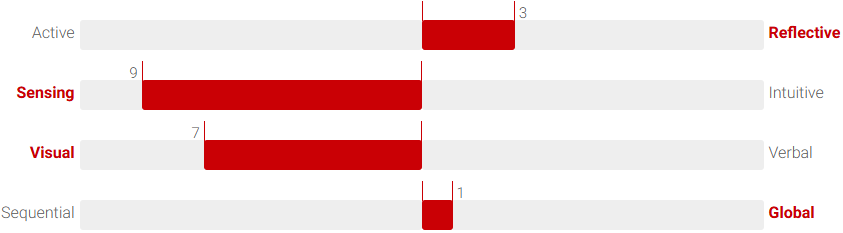
\includegraphics[width=1\linewidth]{Figures/Section_4/ILS_result}
    \caption{Ergebnisse des ILS Fragebogens}
\end{figure}

Demnach lässt sich schließen dass der Autor Hänge zu folgenden Dimensionen aufweist.

\begin{itemize}
    \item Ein ausgewogenes Verhältnis der Aktiven/Reflektiven Dimension
    \item Ein starker Hang zum sensorischem Typen 
    \item Ein mäßiger Hang zum visuellen Typen
    \item Ein ausgewogenes Verhältnis der Sequentiellen/Globalen Dimension
\end{itemize}

Die Hänge der einzelnen Lerntypen wird im praktischen Versuch anschließend in Bezugzu den Vor- und Nachteilen für das Erlernen und Anwenden der CT Aspekte und der verschiedenen Paradigmen gesetzt.
Theoretisch sollten die Ausprägungen folgende Folgen haben.

\begin{itemize}
    \item Kein besonderer Vor- oder Nachteil beim Debugging in funktionaler Programmierung (FP), und beim Erlernen von Programmieren in Einzelarbeit generell
    \item Ein Nachteil beim Anwenden von Algorithmischen Denken, und der Erkennung der Zusammenhänge von FP zu mathematischen Funktionen, sowie das innovative Arbeiten mit einem limitierterem Toolset
    \item Ein möglicher mäßiger Vorteil zur Dekomposition aus der Perspektive eines visuellen Lerntypens, sowie zur Abstraktion auf Funktionsebene in der FP
    \item Kein besonderer zusätzlicher Vorteil in Dekomposition aus Perspektive eines Sequentiellen Lerntypens, sowie der generellen Anwendung von FP in einer sequentiellen Lösungsstrategie
\end{itemize}

\subsection{Problembeschreibung}\label{sec:problemdesc}
Um die aufgestellten Thesen zu prüfen, wurde sich entschieden, eine Programmieraufgabe in einem praktischen Teil zu lösen, und alle Erfahrungen, Schwierigkeiten und Probleme in einer Art "Development Diary" zu dokumentieren.
Die Türme von Hanoi wurden hier gewählt, weil die Aufgabe in einem Anfängerkurs mit eigener Aufgabenstellung vertreten war \cite{cis194}, sowie alle Aspekte des CT abdeckt. Die Aufgabenstellung des Kurses CIS 194 wurde hierbei nicht betrachtet, sondern es wurde von Grund auf selbst eine Lösung gefunden.

In dem Problem geht es um drei Holzstäbe, um die unterschiedlich große, runde Holzplatten gestapelt sind. Das Ziel der Lösung ist es, die aufsteigend gestapelten Platten vom Turm ganz links hin zum Turm ganz rechts zu transportieren. Hierbei gelten drei Regeln. Zum einem darf nie mehr als eine Platte gleichzeitig bewegt werden. Eine Platte darf nur bewegt werden, wenn diese die oberste im Stapel ist. Außerdem darf sich eine größere Platte niemals auf einer kleineren befinden.

\begin{figure}[H]
    \centering
    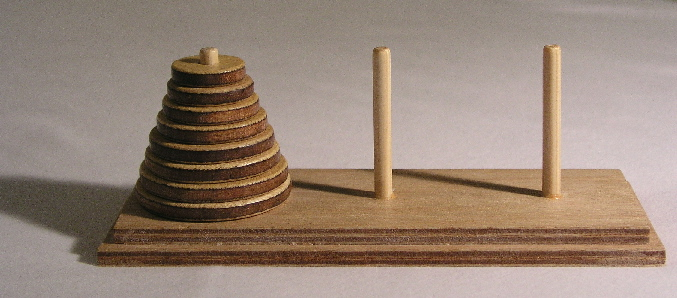
\includegraphics[width=1\linewidth]{Figures/Section_4/hanoi}
    \caption{Ein Modellset der Türme von Hanoi mit 8 Holzplatten \protect\cite{wikicommons}}
\end{figure}

\subsubsection{Theoretische Überlegungen}
Um das Problem zu lösen, wurde zunächst unabhängig vom Code über das Problem nachgedacht. Da ein mäßiger Hang zum visuellen Lerntypen besteht, wurde sich entschieden, das Problem physisch nachzubauen. Diese Methode half besonders dabei, das Problem zu verstehen, und erste Überlegungen zur Abstraktion des Problems durchzuführen. Hierbei war der erste Ansatz, durch zufälliges ausprobieren eine Lösung zu finden. Dies funktionierte zwar einigermaßen, allerdings wurden keine besonderen Muster gefunden, die bei einer allgemeinen Lösung des Problems helfen könnten.

Die ersten tatsächlichen Lösungsansätze waren sehr kompliziert, da noch kein globaleres Verständnis für das Problem vorhanden war. Hierbei wurde zunächst überlegt, wie das Problem abstrahiert werden kann.
Die Holzplatten wurden hierbei als Integer abstrahiert, um einfach die Größen vergleichen zu können. Die Pole selbst wurden als Listen dargestellt, in denen jeweils das erste Element (der "head" der Liste) die oberste Holzplatte darstellt.
Ob eine Bewegung dem legalen Bewegungsset entspricht, wird anhand dessen bestimmt, ob das zu bewegende Element kleiner ist, als das Element auf dem dieses platziert wird. Elemente werden dann so lange bewegt, bis die "Win Condition" erreicht ist, in dem Fall dass sich in den ersten beiden Listen keine Elemente mehr befinden.
Es wurde allerdings schnell bemerkt, besonders als dieser Ansatz anhand des physischen Modells durchgespielt wurden, dass sich schnell unendlichen Schleifen entwickeln. Um einen neuen Ansatz zu finden, wurde deshalb auf Online Visualisierungen zurückgegriffen.

Das Problem wurde zunächst in der simpelsten Form betrachtet, mit insgesamt drei Holzplatten. Hierbei wurde beobachtet, dass das erste "Teilziel" des Problemes ist, die größte Platte zunächst auf den rechten Pol zu setzen. Die anderen Platten werden durch einige Hilfsschritte geordnet in der Mitte platziert. Dieser Ansatz half stark dabei, Muster in der Lösung zu erkennen.

Erst hier wurde richtig verarbeitet, wie das Problem rekursiv gelöst werden kann. Wenn mehr als 3 Holzplatten vorhanden sind, kann das Problem so lange weiter reduziert werden, bis nur noch drei Platten betrachtet werden. Von dort aus kann man das Problem rekursiv mit n-1 Platten lösen.

\subsubsection{Abstraktion}

Da die Funktion rekursiv laufen soll, muss diese alle nötigen Parameter annehmen. Hierzu gehört der Startpol, der Zielpol, und falls nötig ein Hilfspol, auf dem Platten zwischenplatziert werden können. Zudem wird die Anzahl von Holzplatten benötigt, die sich in jedem rekursiven Schritt reduzieren soll. Die Pole selbst werden als Listen mit Integern definiert.
Um die Schritte zur Lösung zu dokumentieren wird zudem eine Liste von Lösungsschritten übergeben, die jeweils in einem Tupel den Startpol, sowie den Endpol komplett dokumentiert. Diese Liste von Lösungsschritten repräsentiert letztendlich die finale Lösung, und ist eine Anleitung zur Lösung des Problems.

Es gibt im Problem selbst nicht allzu viele Teilverantwortlichkeiten, da der größte Teil der Arbeit durch den rekursiven Schritt geschieht. Allerdings lässt sich im Vergleich zu herkömmlichen, nicht funktionale Lösungen sagen, dass das Erstellen und Füllen der Liste mit Lösungsschritten ein zusätzlicher Aspekt ist, der in einer funktionalen lösung berücksichtigt werden muss. Die Schritte können nicht etwa einfach in der Konsole "zwischengedruckt" werden, da Funktionen in der FP pur sind und demnach keine Seiteneffekte haben dürfen.

\subsection{Umsetzung}

Die Umsetzung des Problems im funktionalen Paradigma erfolgte in Haskell. Nachdem das Problem aureichend theoretisch analysiert wurde, wurde überlegt, wie es funktional umsetzbar ist.

\subsection{Zusammenhang mit Lerntypen}
Beim Bearbeiten der Aufgabe wurden einige Beobachtungen speziell im Zusammenhang mit der Forschung aus Abschnitt 3 der Arbeit gemacht. Es wurde angenommen, dass besonders Vorteile in der Dekomposition und Abstraktion auftreten werden, allerdings Schwierigkeiten beim Finden der Algorithmik und der Zusammenhänge der Teilprobleme.

Die Beobachtungen, die in dem praktischen Versuch gemacht wurden, können diese Annahmen stützen. Der Prozess der theoretischen Lösungsfindung, das aufteilen den Problemes in Teilprobleme, sowie die Abstraktionsphase waren alles Aspekte, die relativ einfach waren. Die Schwierigkeiten traten in der Findung des tatsächlichen Algorithmus, sowie der Erkennens des globalen Zusammenhanges auf. Besonders erkennbar waren diese Probleme in der Phase, in der sich mit der Musterfindung beschäftigt wurde, insbesondere der Frage, wie man den Algorithmus allgemein und rekursiv gestalten kann.
